\subsection{Model Performance}
By using the solutions, that we found we can make a prediction for every value of t. Once we have made the predictions, we can then find the error using the RMS error. The RMS error is calculated using the formula $\sqrt{\sum{\frac{1}{27}(v_{actual} - v_{predicted})^2}}$ or by using the formula $\sqrt{\sum{\frac{1}{27}(d_i)^2}}$ . Once the RMS is calculated it can be used to compare the performance of the model, and how it compares to the other improved models.
\\ \\
\begin{table}[H]
\centering
    \begin{tabular}{|l|l|l|l|l|l|l|l|l|l|l|l|l|l|l|l|l|}
        \hline
        t(s) & 0 & 1 & 2 & 3 & 4 & 5 & 6 & 7 & 8 & 9 \\ \cline{1-11} 
        predicted v(m/s) & 96.00 & 91.44 & 86.89 & 82.33 & 77.78 & 73.22 & 68.67 & 64.11 & 59.56 & 55.00\\ \cline{1-11}
        Actual v(m/s) & 96 & 89 & 82 & 77 & 72 & 68 & 64 & 61 & 58 & 55 \\ \cline{1-11}
        $d^2$ & 0.00 & 5.98 & 23.90 & 28.44 & 33.38 & 27.27 &	21.78 & 9.68 & 2.42 & 0.00 \\ \cline{1-11}
    \end{tabular}
    \caption{Case 1}
    \vspace{0.5cm}
    
    \begin{tabular}{|l|l|l|l|l|l|l|l|l|l|l|l|}
        \hline
        t(s) & 10 & 11 & 12 & 13 & 14 & 15 & 16 & 17 & 18 \\ \cline{1-10}
        predicted v(m/s) & 51.76 & 48.53 & 45.29 & 42.06 & 38.82 & 35.59 & 32.35 & 29.12 & 25.88 \\ \cline{1-10}
        Actual v(m/s) & 50 & 46 & 41 & 38 & 34 & 31 & 27 & 24 & 21 \\ \cline{1-10}
        $d^2$ & 3.11 & 6.40 & 18.44 & 16.47 & 23.27 & 21.05 & 28.65 & 26.19 & 23.84 \\ \cline{1-10}
    \end{tabular}
    \caption{Case 2}
    \vspace{0.5cm}
    
    \begin{tabular}{|l|l|l|l|l|l|l|l|l|}
        \hline
        t(s) & 19 & 20 & 21 & 22 & 23 & 24 & 25 & 26 \\ \cline{1-9}
        predicted v(m/s) & 22.65 & 19.41 & 16.18 & 12.94 & 9.71 & 6.47 & 3.24 & 0.00 \\ \cline{1-9}
        Actual v(m/s) & 18 & 16 & 13 & 10 & 8 & 5 & 3 & 0
        \\ \cline{1-9}
        $d^2$ & 21.60 & 11.64 & 10.09 & 8.65 & 2.91 & 2.16 & 0.06 & 0.00 \\ \cline{1-9}
    \end{tabular}
    \caption{Case 2 continued}
    \vspace{0.5cm}
\end{table}

\begin{figure}[H]
\centering
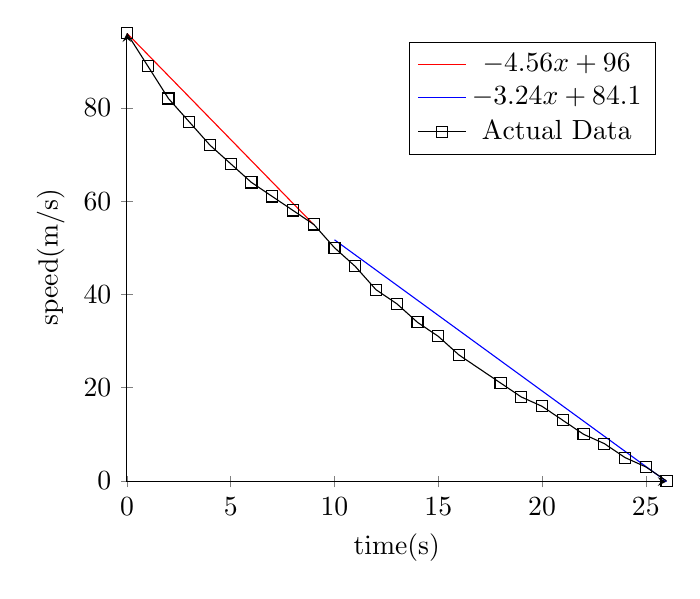
\begin{tikzpicture}
\begin{axis}[
    axis lines = left,
    xlabel = time(s),
    ylabel = speed(m/s),
]
%Below the red parabola is defined
\addplot [
    domain=0:9,
    samples=100, 
    color=red,
]
{-4.56*x + 96};
\addlegendentry{$-4.56x + 96$}
%Here the blue parabloa is defined
\addplot [
    domain=10:26, 
    samples=100, 
    color=blue,
    ]
    {-3.24*x + 84.1};
\addlegendentry{$-3.24x + 84.1$}
 
 \addplot[
    color=black,
    mark=square]
    coordinates {(0,96)(1,89)(2,82)(3,77)(4,72)(5,68)(6,64)(7,61)(8,58)(9,55)(10,50)(11,46)(12,41)(13,38)(14,34)(15,31)(16,27)(18,21)(19,18)(20,16)(21,13)(22,10)(23,8)(24,5)(25,3)(26,0)};
\addlegendentry{Actual Data}
\end{axis}
\end{tikzpicture}
\caption{Graph showing the predicted velocity values against the actual velocity values}
\end{figure}